\documentclass[twoside,11pt]{article}

% Any additional packages needed should be included after jmlr2e.
% Note that jmlr2e.sty includes epsfig, amssymb, natbib and graphicx,
% and defines many common macros, such as 'proof' and 'example'.
%
% It also sets the bibliographystyle to plainnat; for more information on
% natbib citation styles, see the natbib documentation, a copy of which
% is archived at http://www.jmlr.org/format/natbib.pdf

% Available options for package jmlr2e are:
%
%   - abbrvbib : use abbrvnat for the bibliography style
%   - nohyperref : do not load the hyperref package
%   - preprint : remove JMLR specific information from the template,
%         useful for example for posting to preprint servers.
%
% Example of using the package with custom options:
%
% \usepackage[abbrvbib, preprint]{jmlr2e}

\usepackage{jmlr2e}
\graphicspath{{imgs/}}

% Definitions of handy macros can go here

\newcommand{\dataset}{{\cal D}}
\newcommand{\fracpartial}[2]{\frac{\partial #1}{\partial  #2}}

% Heading arguments are {volume}{year}{pages}{date submitted}{date published}{paper id}{author-full-names}

\jmlrheading{21}{2020}{1-48}{4/00}{10/00}{meila00a}{Marina Meil\u{a} and Michael I. Jordan}

% Short headings should be running head and authors last names

\ShortHeadings{OpenPose-Plus}{Meil\u{a} and Jordan}
\firstpageno{1}

\begin{document}

\title{OpenPose-Plus: Flexible Real-time Human Pose Estimation}

\author{\name Marina Meil\u{a} \email mmp@stat.washington.edu \\
       \addr Department of Statistics\\
       University of Washington\\
       Seattle, WA 98195-4322, USA
    %   \AND
    %   \name Michael I.\ Jordan \email jordan@cs.berkeley.edu \\
    %   \addr Division of Computer Science and Department of Statistics\\
    %   University of California\\
    %   Berkeley, CA 94720-1776, USA
       }

\editor{Kevin Murphy and Bernhard Sch{\"o}lkopf}

\maketitle

\begin{abstract}%   <- trailing '%' for backward compatibility of .sty file
%This paper describes the mixtures-of-trees model, a probabilistic 
%model for discrete multidimensional domains.  Mixtures-of-trees 
%generalize the probabilistic trees of \citet{chow:68}
%in a different and complementary direction to that of Bayesian networks.
%We present efficient algorithms for learning mixtures-of-trees 
%models in maximum likelihood and Bayesian frameworks. 
%We also discuss additional efficiencies that can be
%obtained when data are ``sparse,'' and we present data 
%structures and algorithms that exploit such sparseness.
%Experimental results demonstrate the performance of the 
%model for both density estimation and classification. 
%We also discuss the sense in which tree-based classifiers
%perform an implicit form of feature selection, and demonstrate
%a resulting insensitivity to irrelevant attributes.
\end{abstract}

\begin{keywords}
  Pose Estimation, Computer Vision, Real-time Systems
\end{keywords}

\section{Introduction}

%% 应用简介
Human pose estimation is a core task in computer vision.
Its goal is to localise human anatomical key-points (e.g., elbow, wrist, etc.)
and use the detected key-points to infer the pose topology. 
Estimating human pose has many useful applications, such as interactive gaming~\citep{x}, automated supermarket~\citep{x}, motion capture~\citep{x} and self-driving cars~\citep{x}. Usually, users design the pose estimation pipeline and train the Deep Neural Networks(DNNs) on servers and then deploy the pipeline on standalone machines.

%% 痛点
Many practitioners have shown strong interests in applying 
pose estimation techniques in the real world. 
They, however, report two major challenges in the model training and deployment of pose estimation algorithms: (1) \emph{Flexibility}.
The pose estimation pipeline is more complex than other computer vision tasks(e.g., image classification). Different applications involve in different DNN models~\citep{x1, x2, x3}, pre-processing/post-processing methods~\citep{x1, x2, x3} and training datasets\citep{x1, x2, x3};
(2) \emph{Real-time performance}. It is also challenging to achieve real-time data processing required by most pose estimation applications. These applications produce high-resolution images at high rates (e.g., [....]). Processing such data in real time is non-trivial for systems like the robotic systems which have limited computing power due to the limited volume and battery capacity. The real-time pose estimation scenario also faces data IO, CPU and GPU, where proper parallel scheduling should be applied to further improve the performance.

%% 简述现状和相关工作以加深痛点
The state-of-the-art DNN frameworks(e.g., TensorFlow\citep{x}) did not provide other diverse functionalities(e.g., post-processinng) in the pose estimation pipeline. Hence, serveral projects(e.g., OpenPose\citep{x}, AlphaPose\citep{x}) were hard coded to do human pose estimations. However, they're mostly designed to support one specific pose estimation pipeline and none of them provide the required flexibility and real-time performance at the same time. 
On the one hand, oftentimes researchers cannot customize their own pose estimation pipelines based on the current systems and have to write a new framework from scratch, which involves in high development cost. On the other hand, as the current frameworks are mostly built for research usage and model training, it is hard for engineers to reuse the frameworks to deploy their applications with high performance.
% Concrete example建议放到related works里。

% On one extreme, systems like OpenPose~\citep{x}
% are designed for specific pose estimation tasks and hardware architectures.
% They have monolithic optimised system components,
% and do not have principle APIs to alter the choices of 
% data modules and neural networks, making
% them rigid and brittle to be adapted.
% On the other extreme, users can quickly prototype
% pose estimation applications~\citep{x1, x2}
% using general-purpose 
% CPU/GPU engines such as TensorFlow\citep{x} and PyTorch\citep{x}. 
% The performance of these systems is ultimately
% limited by their comprehensive usages of high-level dynamic
% languages (i.e., Python) and the lack of designs for
% efficient execution on embedded platforms.

%% 简述贡献
To close this gap, we argue that: to achieve both flexibility and real-time performance in human pose estimation, it is important to co-design algorithm and their execution runtime. To demonstrate this, we design and develop: OpenPose-Plus, a flexible real-time pose estimation framework. The design of OpenPose-Plus makes two key contributions: it proposes
(i) Neat abstractions and high-level Python and C++(for deployment) APIs which allow users to deeply customize the development and deployment of human pose estimation pipeline, and (ii) a real-time and portable runtime library which is highly optimized by utilizing high-performance DNN inference library: TensorRT, and streaming data processing pipeline to fully parallel the computation devices (i.e., CPUs and GPUs) and data IO.

%% 评估
OpenPose-Plus was open-sourced in October 2018 under a Apache 2 licence. Since after, it has attracted numerous industry and academic users, and has a quickly growing user base on Github (over 700 stars by the date of submission). 

\section{Framework Design and Implementation}

The design of OpenPose-Plus includes development and deployment two parts. In development side, OpenPose-Plus aims at helping data scientists train and evaluate diverse DNN models over large datasets with ease. Hence, the development part is designed for flexibility, modularization and user friendliness. In the deployment side, the target users are mainly software engineers, and real-time video/camera data processing is the key challenge and requirement. The deployment part of OpenPose-Plus utilizes fine-grained parallelism and elegant abstraction to achieve the goal of high performance, flexibility and portability in real-time pose estimation applications. Then the two parts can collaborate seamlessly using the provided model conversion utility.

\subsection{Modularized Uniform Training}

The training component of OpenPose-Plus mainly contains three modules: \texttt{Model}, \texttt{Dataset} and \texttt{Config} (Figure \ref{fig:ModuleAPI}). Each module provides unified simple APIs with the purpose of making the construction process over different model architectures, datasets and configurations convenient and thus relieves users from spending time over trivial but exhausting procedures rather than the critical model design and analysis.

\textbf{Multi-model architecture:}
To tackle the challenge that different models represent human body key points and topology in distinct ways, OpenPose-Plus abstracts classic model classes that covers most of the existing popular models into a single module \texttt{Model}. For each class, OpenPose-Plus provides an integral pipeline of data preprocessing, training, evaluation and visualization in  consistent APIs. Users can easily employ the corresponding procedures so that they can put the main focus on network architecture design and model performance comparison observing the visualized output. 

\textbf{Multi-dataset interface:}
To generalize models on various application scenes, it is always desired to train and evaluate the model on several datasets with distinctive distributions. But the definition and the form of annotations differ a lot between existing datasets. Again, Openpose-plus abstract a wide range of popular datasets into the module \texttt{Dataset} which offers APIs to generate uniformly formatted data pairs that could be directly used, while also allow users to filter the data in their own need and visualize the annotations. 

\textbf{Flexible configuration:}
The configuration of the model means a lot, some have an impact on model performance (e.g., learning rate), while some affect training efficiency and depend on the hardware resources (e.g., batch size). This leads to the need of dynamic configuration to adapt to the current optimization target and available devices. Openpose-plus copes with this by first introducing module \texttt{Config} with abundant APIs for users to dynamically adjust the static general configuration and assemble the configured parts into a whole system with flexibility. Then the high-performance distributed training library Kungfu is integrated to offer parallel training option which enables users to make full use of hardware resources to train the model much more efficiently when in need.


\begin{figure}[h]
\centering
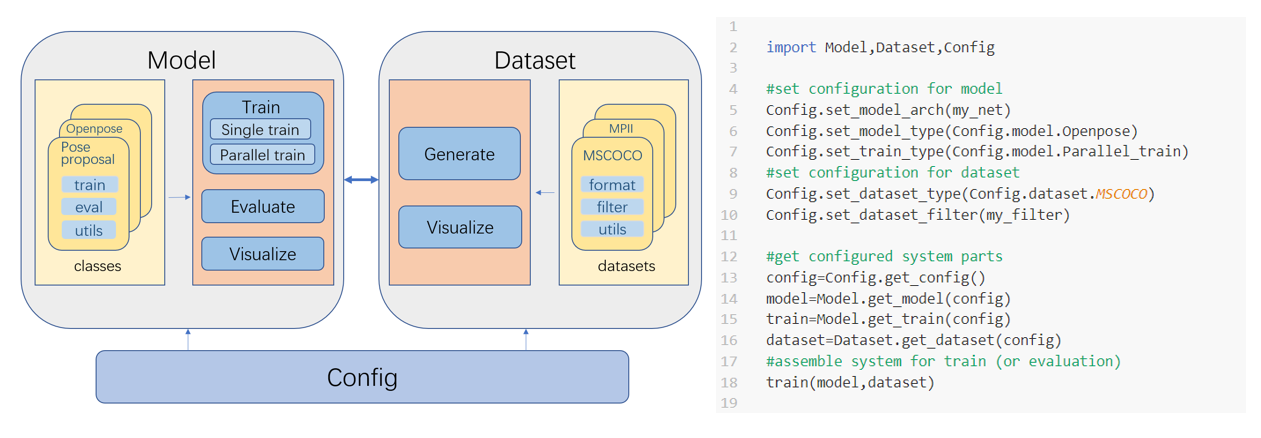
\includegraphics[width=0.9\linewidth]{ModuleAPI.png}
\caption{The train modules and code sample of the module API. }
\label{fig:ModuleAPI}
\end{figure}

\subsection{High-Performance Runtime Processing}

The runtime processing pipeline of OpenPose-Plus can usually be divided into 2 components: DNN inference and post processing. In the DNN inference stage, OpenPose-Plus utilizes TensorRT\citep{x} to inference the input image to generate feature maps(i.e. activation maps) on GPU. And in the post processing stage, OpenPose-Plus parses the feature maps to find out the location of key points and the pose topology on CPU.

The targets of OpenPose-Plus runtime processing API design is to provide both the out-of-the-box(OOTB) usage experience and the access to the underlying data manipulations, while maintaining high performance. Hence, OpenPose-Plus provides 2 levels of APIs: the fine-grained \textbf{operator API} to conduct the DNN inference and post processing and the OOTB \textbf{stream API}(Figure \ref{fig:StreamAPI}) for stream-like data processing.

In the operator API, users can use DNN inference module to generate feature maps by providing the model parameter files, and extract the pose topology by simply selecting the corresponding feature map parser. The operator API are very portable that users can easily make use of in pose estimation applications to conduct fine-grained operations. Based on operator API, the stream API provides a high-level abstraction while achieving better performance. Users only need to specify the DNN model, parser type and input/output streams using the stream API.(e.g., image sequence, video, camera stream, etc.)

In the stream design setting(Figure \ref{fig:StreamAPI}), data is transmitted in streams(FIFO queue). In the first module, OpenPose-Plus conducts preprocessing(i.e., resize) and packs queued images into batches to conduct fast batch processing on GPU(batch processing is more efficient than single-frame processing) and push the generated feature maps into the inner stream. In the meanwhile, the post-processing module utilizes multi-threading to parse the feature maps simultaneously and the results were written into output files (e.g., video) in the output stream. 

The streaming implementation can achieves ?x speedup compared with the non-streaming pipelining implementation.

\begin{figure}[h]
\centering
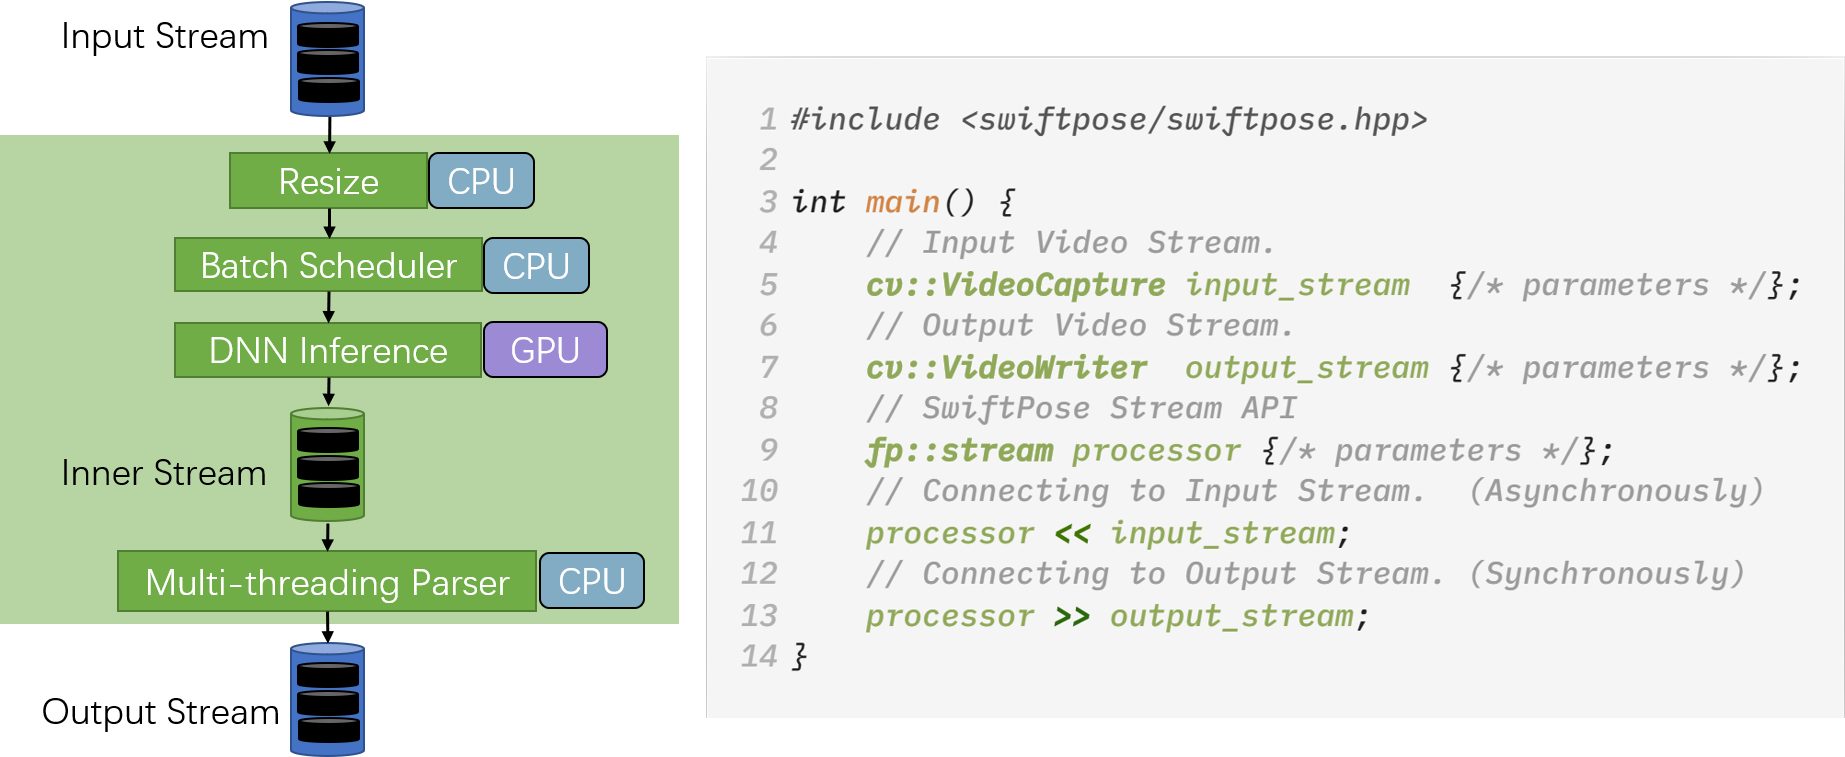
\includegraphics[width=0.85\linewidth]{StreamAPI.png}
\caption{The processing architecture and code sample of the stream API.}
\label{fig:StreamAPI}
\end{figure}

% \section{High-level APIs and Applications}

% \subsection{Training APIs}
% The bottom details of different models, datasets and configurations varies a lot, usually complicated and exhausting to implement.
% The targets of Openpose-Plus train API design is to offer unified simple interfaces over these details to relieve users from spending considerable time on numerous trivial procedures rather than focusing on model design and analysis. 

% The train APIs distribute in the three modules.(Figure \ref{fig:ModuleAPI})
% The \textbf{Model API} provides functions for each class of models including train, evaluation and visualization etc, which cover most of the procedure that building a model prototype needs.
% The \textbf{Dataset API} offers uniformly formatted data pairs, while also allow users to filter the data in their need and visualize the annotations.
% The \textbf{Config API} contains most of the interfaces that give user a great flexibility to configure each part of the system and then assemble them to run.


% \subsection{Runtime Processing APIs}\label{RuntimeAPI}

% Pose estimation applications involve in different types of media data(e.g., videos, images), DNN models and corresponding post processings, which is a big challenge to maintain both good abstraction and performance. 

% The targets of OpenPose-Plus runtime processing API design is to provide both the out-of-the-box(OOTB) usage experience and the access to the underlying data manipulations, while maintaining high performance. Hence, OpenPose-Plus provides 2 levels of APIs: the fine-grained \textbf{operator API} to conduct the DNN inference and post processing and the OOTB \textbf{stream API}(Figure \ref{fig:StreamAPI}) for stream-like data processing.

% In the operator API, users can use DNN inference module to generate feature maps by providing the model parameter files, and extract the pose topology by simply selecting the corresponding feature map parser. The operator API are very portable that users can easily make use of in pose estimation applications to conduct fine-grained operations. Based on operator API, the stream API provides a high-level abstraction while achieving better performance. Users only need to specify the DNN model, parser type and input/output streams using the stream API.(e.g., image sequence, video, camera stream, etc.)

\section{Comparison against Related Works}

% TODO: Comparison about training. (建议可以说说在基础的训练框架上后处理部分没有被实现,而他们又很难写hard code)
% TODO: Comparison analysis.
% We evaluate the effectiveness of OpenPose-Plus using extensive application studies and test-bed performance evaluation. Application study shows that the high-level APIs of OpenPose-Plus are sufficient to implement various pose estimation applications, including [...], which are difficult to release today. OpenPose-Plus is also able to achieve real-time data processing on today's commodity embedded platforms. Specifically, it can process [...] images per second on [...], [...] and [...] faster
% than the state-of-the-art: OpenPose and [...], respectively. 

In table \ref{table:Benchmark}, we show the benchmark\footnote{Benchmark environment: Ubuntu 18.04, with 6 core Intel CPU and 1070Ti NVIDIA GPU.} of different pose estimation across different frameworks.

\begin{tabular}{ |p{3.8cm}||p{2.7cm}|p{1.9cm}|p{1.9cm}|p{2.7cm}|}
 \hline
 \multicolumn{5}{|c|}{\textbf{Benchmarks}} \\
 \hline
 Method              & OpenPose-Plus &OpenPose&TensorFlow&References\\
 \hline
OpenPose             &?              &?       &?         &\citep{x}\\
Lightweight OpenPose &?              &?       &?         &\citep{x}\\
Proposal Network     &?              &?       &?         &\citep{x}\\
 \hline
\end{tabular}\label{table:Benchmark}

\section{Future Works}
% TODO
@Brother Milo@Brother Hao.

more hardware

3D models


% Acknowledgements should go at the end, before appendices and references

%\acks{We would like to acknowledge support for this project
%from the National Science Foundation (NSF grant IIS-9988642)
%and the Multidisciplinary Research Program of the Department
%of Defense (MURI N00014-00-1-0637). }

% Manual newpage inserted to improve layout of sample file - not
% needed in general before appendices/bibliography.

%\newpage

%\appendix
%\section*{Appendix A.}
%\label{app:theorem}
%
%% Note: in this sample, the section number is hard-coded in. Following
%% proper LaTeX conventions, it should properly be coded as a reference:
%
%%In this appendix we prove the following theorem from
%%Section~\ref{sec:textree-generalization}:
%
%In this appendix we prove the following theorem from
%Section~6.2:
%
%\noindent
%{\bf Theorem} {\it Let $u,v,w$ be discrete variables such that $v, w$ do
%not co-occur with $u$ (i.e., $u\neq0\;\Rightarrow \;v=w=0$ in a given
%dataset $\dataset$). Let $N_{v0},N_{w0}$ be the number of data points for
%which $v=0, w=0$ respectively, and let $I_{uv},I_{uw}$ be the
%respective empirical mutual information values based on the sample
%$\dataset$. Then
%\[
%	N_{v0} \;>\; N_{w0}\;\;\Rightarrow\;\;I_{uv} \;\leq\;I_{uw}
%\]
%with equality only if $u$ is identically 0.} \hfill\BlackBox
%
%\noindent
%{\bf Proof}. We use the notation:
%\[
%P_v(i) \;=\;\frac{N_v^i}{N},\;\;\;i \neq 0;\;\;\;
%P_{v0}\;\equiv\;P_v(0)\; = \;1 - \sum_{i\neq 0}P_v(i).
%\]
%These values represent the (empirical) probabilities of $v$
%taking value $i\neq 0$ and 0 respectively.  Entropies will be denoted
%by $H$. We aim to show that $\fracpartial{I_{uv}}{P_{v0}} < 0$....\\
%
%{\noindent \em Remainder omitted in this sample. See http://www.jmlr.org/papers/ for full paper.}


% \vskip 0.2in
\newpage
\bibliography{sample}

\end{document}
